\documentclass[12pt]{article}
\usepackage[english]{babel}
\usepackage{fancyhdr}
\usepackage{hyperref}
\usepackage{indentfirst}
\usepackage{underscore}
\usepackage{graphicx}


\pagestyle{fancy}
\fancyhf{}
\fancypagestyle{plain}{%
	\fancyhf{}%
	\fancyhf[CH]{Richard Sindely}%
	\fancyhf[CF]{AxAi}%
	\fancyhf[RF]{\thepage}%
}
\renewcommand{\footrulewidth}{0.4pt}
\fancyhf[CH]{Richard Sindely}
\fancyhf[CF]{AxAi}
\fancyhf[RF]{\thepage}

\author{Richard Sindely}
\title{AxAi documentation}
\date{2025}

\begin{document}
\maketitle
\newpage
\tableofcontents
\newpage
\section{Introduction}
\label{int}

This program is a task assigned by AgileXpert, this includes the basic tasks and the assignments for AI role applicants. You can access the tasks description \href{https://agilexpert.hu/megoldando-problema-leirasa/}{here}.
\subsection{Technical information}

The application is written in Java using the Spring Boot framework and communicates with the user through a Command-Line Interface (CLI). It includes an AI feature that allows the user to request command execution through natural language.

The backend uses a MySQL database. Hibernate (JPA) is used to handle data storage, so there is no need to write raw SQL queries manually.

The data model is implemented using classes annotated with @Entity, which marks them as JPA entities mapped to the database tables.
In some cases, the @Transactional annotation was necessary to access data from related tables due to issues with lazy loading. Using eager fetching would be a solution, but it would load unnecessary data that could lead to inefficient resource usage. UUIDs are used in the project because the chance of generating duplicates is extremely low. UUIDs are automatically generated for all entities.

The SQL command for user creation can be found in the README.md. It is required in order to connect to the database. The application automatically creates a database named axaidb if it does not already exist.

The AI feature calls the OpenAI API, which returns a command to be executed. The application requires an API KEY, which can be added to the root directory in a file named "openai.env".

\subsection{Setup}
\begin{itemize}
	\item Clone the project.
	\item Install MySQL.
	\item Create a MySQL user (read the README.md for the command).
	\item Run the application by executing mvn spring-boot:run in the root directory of the project.
\end{itemize}
\newpage
\section{Database}
\subsection{Entities}
User entity:
\begin{itemize}
	\item id (PK)
	\item username
	\item password (Passwords are stored in a hashed format.)
	\item theme_id (User's theme)
	\item selected_background_id (FK)
	\item menu_id (FK)
\end{itemize}
Background entity
\begin{itemize}
	\item id (PK)
	\item name (background's name)
	\item user_id (FK)
\end{itemize}
Menu entity
\begin{itemize}
	\item id (PK)
	\item name
\end{itemize}
SubMenu entity
\begin{itemize}
	\item id (PK)
	\item name (Submenu's name)
	\item menu_id (FK)
\end{itemize}
Submenu-App relationship table:
\begin{itemize}
	\item submenu_id (FK)
	\item app_id (FK)
\end{itemize}
Theme entity
\begin{itemize}
	\item id (PK)
	\item name (Theme's name)
\end{itemize}
App entity
\begin{itemize}
	\item id (PK)
	\item icon_name
	\item name (App's name)
	\item user_id (FK)
\end{itemize}
\subsection{ER diagram}
\begin{figure}[h!]
	\centering
	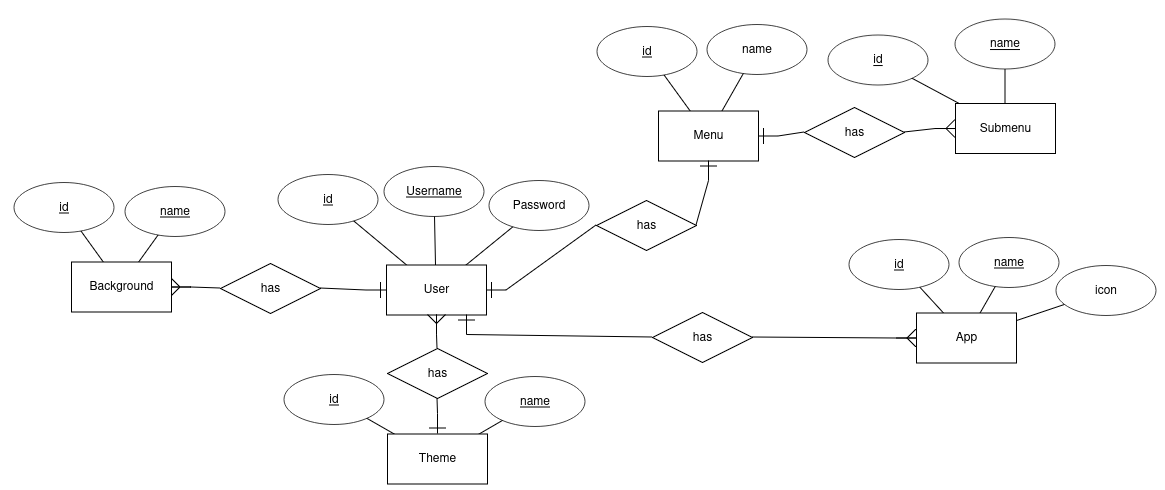
\includegraphics[width=1.2\textwidth]{er_model.png}
\end{figure}
\newpage
\subsection{RS diagram}
\begin{figure}[h!]
	\centering
	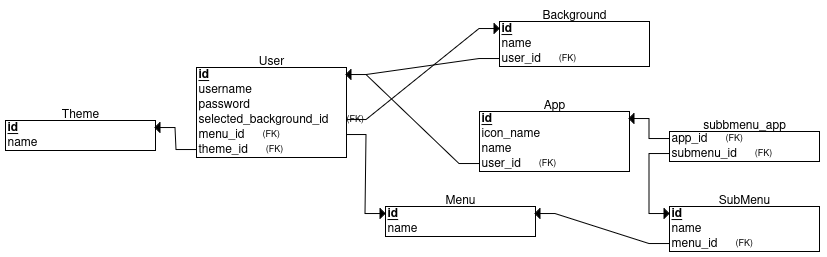
\includegraphics[width=1.2\textwidth]{rs.png}
\end{figure}

\section{Structure}
The project uses a repository layer to interact with the database. The service layer communicates with the repositories to retrieve, update, and manage data. These repositories are annotated with @Repository,the services with @Service, and each entity has a corresponding repository interface. 

The application currently uses a CLI interface, but a controller can be added later if a frontend is needed.

\newpage

\section{Commands}
If the user is not logged-in:
\begin{itemize}
	\item Create a user: create-user userName password
	\item Login: login
	\item Exit: exit:
\end{itemize}
If the user is logged-in:
\begin{itemize}
	\item Logout: logout
	\item Exit: exit
	\item Edit your username: rename-user newName passwd
	\item Change your password: change-password password newPassword
	\item Delete your user: delete-user passwd
	\item List your menu:menu
	\item Create new submenu: create-menu menuName
	\item Rename submenu: rename-menu oldName NewName
	\item Delete submenu: delete-menu menuName
	\item Add app to submenu: add-app menuName appName
	\item Remove app from submenu: remove-app-menu menuName appName
	\item Create app: download-app appName iconName
	\item Delete app: delete-app appName
	\item Update app icon: update-app-icon appName newIconName
	\item Delete app icon: delete-app-icon appName
	\item Run an app: run-app appName
	\item Set your theme: set-theme themeName
	\item Add theme: add-theme themeName
	\item Add background: add-background backgroundName
	\item Choose background: set-background backgroundName
\end{itemize}
\end{document}